% Options for packages loaded elsewhere
\PassOptionsToPackage{unicode}{hyperref}
\PassOptionsToPackage{hyphens}{url}
\PassOptionsToPackage{dvipsnames,svgnames,x11names}{xcolor}
%
\documentclass[
  letterpaper,
  DIV=11,
  numbers=noendperiod]{scrartcl}

\usepackage{amsmath,amssymb}
\usepackage{iftex}
\ifPDFTeX
  \usepackage[T1]{fontenc}
  \usepackage[utf8]{inputenc}
  \usepackage{textcomp} % provide euro and other symbols
\else % if luatex or xetex
  \usepackage{unicode-math}
  \defaultfontfeatures{Scale=MatchLowercase}
  \defaultfontfeatures[\rmfamily]{Ligatures=TeX,Scale=1}
\fi
\usepackage{lmodern}
\ifPDFTeX\else  
    % xetex/luatex font selection
\fi
% Use upquote if available, for straight quotes in verbatim environments
\IfFileExists{upquote.sty}{\usepackage{upquote}}{}
\IfFileExists{microtype.sty}{% use microtype if available
  \usepackage[]{microtype}
  \UseMicrotypeSet[protrusion]{basicmath} % disable protrusion for tt fonts
}{}
\makeatletter
\@ifundefined{KOMAClassName}{% if non-KOMA class
  \IfFileExists{parskip.sty}{%
    \usepackage{parskip}
  }{% else
    \setlength{\parindent}{0pt}
    \setlength{\parskip}{6pt plus 2pt minus 1pt}}
}{% if KOMA class
  \KOMAoptions{parskip=half}}
\makeatother
\usepackage{xcolor}
\setlength{\emergencystretch}{3em} % prevent overfull lines
\setcounter{secnumdepth}{5}
% Make \paragraph and \subparagraph free-standing
\makeatletter
\ifx\paragraph\undefined\else
  \let\oldparagraph\paragraph
  \renewcommand{\paragraph}{
    \@ifstar
      \xxxParagraphStar
      \xxxParagraphNoStar
  }
  \newcommand{\xxxParagraphStar}[1]{\oldparagraph*{#1}\mbox{}}
  \newcommand{\xxxParagraphNoStar}[1]{\oldparagraph{#1}\mbox{}}
\fi
\ifx\subparagraph\undefined\else
  \let\oldsubparagraph\subparagraph
  \renewcommand{\subparagraph}{
    \@ifstar
      \xxxSubParagraphStar
      \xxxSubParagraphNoStar
  }
  \newcommand{\xxxSubParagraphStar}[1]{\oldsubparagraph*{#1}\mbox{}}
  \newcommand{\xxxSubParagraphNoStar}[1]{\oldsubparagraph{#1}\mbox{}}
\fi
\makeatother


\providecommand{\tightlist}{%
  \setlength{\itemsep}{0pt}\setlength{\parskip}{0pt}}\usepackage{longtable,booktabs,array}
\usepackage{calc} % for calculating minipage widths
% Correct order of tables after \paragraph or \subparagraph
\usepackage{etoolbox}
\makeatletter
\patchcmd\longtable{\par}{\if@noskipsec\mbox{}\fi\par}{}{}
\makeatother
% Allow footnotes in longtable head/foot
\IfFileExists{footnotehyper.sty}{\usepackage{footnotehyper}}{\usepackage{footnote}}
\makesavenoteenv{longtable}
\usepackage{graphicx}
\makeatletter
\def\maxwidth{\ifdim\Gin@nat@width>\linewidth\linewidth\else\Gin@nat@width\fi}
\def\maxheight{\ifdim\Gin@nat@height>\textheight\textheight\else\Gin@nat@height\fi}
\makeatother
% Scale images if necessary, so that they will not overflow the page
% margins by default, and it is still possible to overwrite the defaults
% using explicit options in \includegraphics[width, height, ...]{}
\setkeys{Gin}{width=\maxwidth,height=\maxheight,keepaspectratio}
% Set default figure placement to htbp
\makeatletter
\def\fps@figure{htbp}
\makeatother
% definitions for citeproc citations
\NewDocumentCommand\citeproctext{}{}
\NewDocumentCommand\citeproc{mm}{%
  \begingroup\def\citeproctext{#2}\cite{#1}\endgroup}
\makeatletter
 % allow citations to break across lines
 \let\@cite@ofmt\@firstofone
 % avoid brackets around text for \cite:
 \def\@biblabel#1{}
 \def\@cite#1#2{{#1\if@tempswa , #2\fi}}
\makeatother
\newlength{\cslhangindent}
\setlength{\cslhangindent}{1.5em}
\newlength{\csllabelwidth}
\setlength{\csllabelwidth}{3em}
\newenvironment{CSLReferences}[2] % #1 hanging-indent, #2 entry-spacing
 {\begin{list}{}{%
  \setlength{\itemindent}{0pt}
  \setlength{\leftmargin}{0pt}
  \setlength{\parsep}{0pt}
  % turn on hanging indent if param 1 is 1
  \ifodd #1
   \setlength{\leftmargin}{\cslhangindent}
   \setlength{\itemindent}{-1\cslhangindent}
  \fi
  % set entry spacing
  \setlength{\itemsep}{#2\baselineskip}}}
 {\end{list}}
\usepackage{calc}
\newcommand{\CSLBlock}[1]{\hfill\break\parbox[t]{\linewidth}{\strut\ignorespaces#1\strut}}
\newcommand{\CSLLeftMargin}[1]{\parbox[t]{\csllabelwidth}{\strut#1\strut}}
\newcommand{\CSLRightInline}[1]{\parbox[t]{\linewidth - \csllabelwidth}{\strut#1\strut}}
\newcommand{\CSLIndent}[1]{\hspace{\cslhangindent}#1}

\usepackage{booktabs}
\usepackage{longtable}
\usepackage{array}
\usepackage{multirow}
\usepackage{wrapfig}
\usepackage{float}
\usepackage{colortbl}
\usepackage{pdflscape}
\usepackage{tabu}
\usepackage{threeparttable}
\usepackage{threeparttablex}
\usepackage[normalem]{ulem}
\usepackage{makecell}
\usepackage{xcolor}
\usepackage{tabularray}
\usepackage[normalem]{ulem}
\usepackage{graphicx}
\UseTblrLibrary{booktabs}
\UseTblrLibrary{rotating}
\UseTblrLibrary{siunitx}
\NewTableCommand{\tinytableDefineColor}[3]{\definecolor{#1}{#2}{#3}}
\newcommand{\tinytableTabularrayUnderline}[1]{\underline{#1}}
\newcommand{\tinytableTabularrayStrikeout}[1]{\sout{#1}}
\KOMAoption{captions}{tableheading}
\makeatletter
\@ifpackageloaded{caption}{}{\usepackage{caption}}
\AtBeginDocument{%
\ifdefined\contentsname
  \renewcommand*\contentsname{Table of contents}
\else
  \newcommand\contentsname{Table of contents}
\fi
\ifdefined\listfigurename
  \renewcommand*\listfigurename{List of Figures}
\else
  \newcommand\listfigurename{List of Figures}
\fi
\ifdefined\listtablename
  \renewcommand*\listtablename{List of Tables}
\else
  \newcommand\listtablename{List of Tables}
\fi
\ifdefined\figurename
  \renewcommand*\figurename{Figure}
\else
  \newcommand\figurename{Figure}
\fi
\ifdefined\tablename
  \renewcommand*\tablename{Table}
\else
  \newcommand\tablename{Table}
\fi
}
\@ifpackageloaded{float}{}{\usepackage{float}}
\floatstyle{ruled}
\@ifundefined{c@chapter}{\newfloat{codelisting}{h}{lop}}{\newfloat{codelisting}{h}{lop}[chapter]}
\floatname{codelisting}{Listing}
\newcommand*\listoflistings{\listof{codelisting}{List of Listings}}
\makeatother
\makeatletter
\makeatother
\makeatletter
\@ifpackageloaded{caption}{}{\usepackage{caption}}
\@ifpackageloaded{subcaption}{}{\usepackage{subcaption}}
\makeatother

\ifLuaTeX
  \usepackage{selnolig}  % disable illegal ligatures
\fi
\usepackage{bookmark}

\IfFileExists{xurl.sty}{\usepackage{xurl}}{} % add URL line breaks if available
\urlstyle{same} % disable monospaced font for URLs
\hypersetup{
  pdftitle={X-Factors: External Influences of a Hockey Goaltender's Performance},
  pdfauthor={Daniel Du},
  colorlinks=true,
  linkcolor={blue},
  filecolor={Maroon},
  citecolor={Blue},
  urlcolor={Blue},
  pdfcreator={LaTeX via pandoc}}


\title{X-Factors: External Influences of a Hockey Goaltender's
Performance\thanks{Code and data are available at:
\url{https://github.com/danield424/HockeyShotAnalysis}.}}
\usepackage{etoolbox}
\makeatletter
\providecommand{\subtitle}[1]{% add subtitle to \maketitle
  \apptocmd{\@title}{\par {\large #1 \par}}{}{}
}
\makeatother
\subtitle{Higher Team Score Differential, Shot Activity, and Momentum
Boost Goals Saved Above Expected}
\author{Daniel Du}
\date{December 3, 2024}

\begin{document}
\maketitle
\begin{abstract}
This paper investigates how external factors influence hockey
goaltenders' performance during games, using Goals Saved Above Expected
(GSAx) over 10-minute time intervals as the measure of success.
Variables relating to pre-game context, in-game performance, and recent
form are analyzed to understand their impact on performance. Our
findings reveal that goaltenders perform better when their team is
leading and when they are actively engaged, but sustained workloads
negatively affect outcomes. These results provide a clearer
understanding of how game context shapes performance, offering practical
implications for evaluating and optimizing goaltender usage.
\end{abstract}


\section{Introduction}\label{introduction}

Few team sport athletes have as much influence on team performance as
the hockey goaltender. Legendary performances, like Dominik Hasek
single-handedly dragging Czechia past heavy favourites Canada and Russia
to win the 1998 Olympic gold medal, are etched in the history books
forever. Yet up until recently, it was hard to quantify goaltender
performances; standard metrics such as wins, percentage of shots saved,
and goals allowed per game did not tell the full story about
goaltender's performance. The explosion in popularity of sports
analytics has led to new metrics that better measure what fans see with
the eye test. The most popular advanced metric, Goals Saved Above
Expected (GSAx), is an all-encompassing statistic that captures a
goaltender's performance relative to their peers. This is calculated by
finding the difference between the goals a goaltender allows and the
number a goaltender is `expected' to allow; the expectation is
quantified using an advanced model with many factors, such as
MoneyPuck's model Tanner (2024).

Although GSAx is an established metric that outlines which goaltenders
consistently overperform, it still isn't clear \emph{why} they, beyond
obvious factors like skill level and experience. Questions about the
impact of external factors like workload, game state, or recent
engagement remain largely unanswered, with discussions often reduced to
subjective terms like ``mentality'' or ``being on a roll.'' This paper
aims to address these gaps by analyzing the impact of external factors
on a goaltender's GSAx during a game. Specifically, it investigates how
variables relating to game state, in-game performance, and recent form
influence a goaltender's performance within a 10-minute game interval;
the estimand is the magnitude of the effects of these factors. Using a
regression model, we quantify the relationship between these external
variables and performance outcomes, providing a clearer understanding of
what drives overperformance or underperformance.

Our findings show that external factors significantly shape goaltender
performance. Increased shot activity in the preceding three minutes and
positive prior performance as a proxy for momentum are associated with
improved performance, while sustained workloads lead to declines. These
patterns suggest that in-game context is most important in determining
goaltender performance.

The remainder of this paper is structured as follows:
Section~\ref{sec-data} introduces the data and methodology used;
Section~\ref{sec-model} describes the model used to answer our research
question; Section~\ref{sec-results} presents the key findings;
Section~\ref{sec-discussion} discusses the real-world implications of
these results.

\newpage

\section{Data}\label{sec-data}

\subsection{Overview}\label{overview}

To analyze the effect of external factors on goaltender performance, we
use a log of 394,250 shots taken during the 2021-22 to 2024-25 NHL
regular and post-seasons, provided by Moneypuck Tanner (2024). Moneypuck
is a publicly available source of hockey analytics that tracks advanced
statistics, playoff odds, and event data. The shot data is updated daily
from official NHL game reports, and is organized by season. For the
current 2024-25 season, data is included up to November 26, 2024.

The dataset includes well-documented variables essential for analyzing
goaltender performance, and was selected for its reliability,
comprehensive coverage, and accessibility. While other sources, such as
the NHL's API or third-party aggregators like Natural Stat Trick, offer
similar information, Moneypuck's integration of official NHL reporting,
consistent data updates, and easy access make it the preferred choice.
Shot data available for all years since 2008-09; we choose the 2021-22
season as the dataset starting point as this was the first full season
following the COVID-19 pandemic.

The data spans 137 variables that provide metadata and contextual
information about each shot. This analysis focuses on external factors
hypothesized to influence goaltender performance, grouped into
categories related to game state, in-game performance, and recent
performance (see Section~\ref{sec-variables}). Data cleaning steps
ensured consistency and accuracy, with a detailed explanation provided
in Section~\ref{sec-appendix-a}.

The data spans 137 variables that provide metadata and contextual
information about each shot. This analysis focuses on a subset of
variables representing external factors hypothesized to influence
goaltender performance, grouped into categories related to game state,
in-game performance, and recent performance. The data was thoroughly
cleaned to ensure accuracy and prepare it for analysis; the process is
detailed in Section~\ref{sec-appendix-a}.

\subsection{Measurement and Limitations}\label{sec-measurement}

Shots, defined as any player's attempt to score by directing the puck at
the net, are classified as an event type by the NHL. Events, along with
their associated attributes and metadata, are officially recorded by
Sportradar, the NHL's data partner, using AI-powered data tools (2024).
Events are also counted and verified by official scorekeepers.

Both AI and human collection methods are subject to potential errors,
including misclassification or missed events; the exact processes used
to address data discrepancies are not disclosed, introducing a level of
uncertainty. However, the likelihood of significant errors is low given
the importance of accurate statistics to the NHL - statistics are
critical for tracking individual and team performance, determining award
winners, and informing league decisions, such as rule enforcement or
changes. Therefore, Moneypuck's integration of this information provides
a reliable resource for analytics.

\subsection{Variables}\label{sec-variables}

From the cleaned dataset, we calculate response variable
\texttt{GSAx\_segment}, which represents the average goals saved above
expected by a goaltender over a 10-minute segment. Our goal is to
identify external factors that influence a goaltender's performance;
below we outline the reasons for measuring performance with
\texttt{GSAx\_segment}. We select predictor variables representing
external factors hypothesized to affect goaltender performance during
the time interval. These predictors are categorized into three groups:

\begin{enumerate}
\def\labelenumi{\arabic{enumi}.}
\tightlist
\item
  Game state:
\end{enumerate}

\begin{itemize}
\tightlist
\item
  \texttt{isHomeTeam}: Indicates whether the goaltender is playing at
  home or away.
\item
  \texttt{isPlayoffGame}: Indicates whether the game is a regular-season
  or playoff game.
\end{itemize}

\begin{enumerate}
\def\labelenumi{\arabic{enumi}.}
\setcounter{enumi}{1}
\tightlist
\item
  In-game performance and workload: sll of these metrics are measured by
  first finding the value for each shot in a \texttt{GSAx\_segment}
  based on prior shot data, then getting the final value by averaging
  the shot-level values across the segment.
\end{enumerate}

\begin{itemize}
\tightlist
\item
  \texttt{period}: the game period (e.g.~1st, 2nd).
\item
  \texttt{goalieTeamScoreDifferential}: the score differential for the
  goaltender's team (positive when winning, negative when losing).
\item
  \texttt{shots\_faced}: a measure of the total shots the goaltender has
  faced in the game.
\item
  \texttt{shotslast3min}: the shots the goaltender has faced in the last
  3 minutes.
\item
  \texttt{GSAx\_so\_far}: the goaltender's GSAx so far in the game.
\end{itemize}

\begin{enumerate}
\def\labelenumi{\arabic{enumi}.}
\setcounter{enumi}{2}
\tightlist
\item
  Recent games performance:
\end{enumerate}

\begin{itemize}
\tightlist
\item
  \texttt{last\_game\_GSAx}: GSAx from the previous game, representing
  goaltender performance in the previous game.\\
\item
  \texttt{last\_5\_avg\_GSAx}: average GSAx from the 5 previous games,
  representing performance in the previous 5 games.
\end{itemize}

Some pairs of predictors are closely related, such as
\texttt{shots\_faced} and \texttt{shotslast3min}, and
\texttt{last\_game\_GSAx} and \texttt{last\_5\_avg\_GSAx}. Potential
multicollinearity arising from these relationships is addressed in
Section~\ref{sec-model}, where we also explore interactions between
predictors.

Our research focuses on how external circumstances influence goaltender
performance, not the difficulty of the shots themselves. Therefore, we
exclude variables directly used in the calculation of \texttt{GSAx},
such as shot danger and location. These variables measure the intrinsic
difficulty of the shots faced and are already incorporated into
\texttt{GSAx}. Including them as predictors would conflate shot quality
with the external factors we want to analyze, such as game state,
workload, and recent form.

By excluding these variables, we ensure the model evaluates the
situational factors that drive over or underperformance relative to the
expectations set by the shots faced, as captured by
\texttt{GSAx\_segment}.

\subsubsection{Outcome variable}\label{sec-responsevariable}

\texttt{GSAx\_segment} quantifies goaltender performance over 10-minute
time intervals during a game. It is calculated by averaging the Goals
Saved Above Expected (GSAx) of all shots faced by a goaltender within
10-minute chunks of game time. This approach aggregates performance
across several shots to provide a more stable measure of goaltender
ability, minimizing the influence of variability inherent within single
shots. Using time-segmented data, rather than shot-specific values,
allows us to evaluate patterns of performance more reliably across a
game.

Using 10-minute time segments to measure GSAx has limitations, as the
intervals do not align perfectly with the key game events such as
periods of player imbalance or of high shot volume. Furthermore,
segments in games with overtime are cut short due to sudden-death
scoring, potentially biasing its comparability with other segments.
However, \texttt{GSAx\_segment} is still valuable as it balances
granularity and interpretability, providing snapshots of short-term
performance without the noise introduced analyzing shot by shot. It also
allows for uniform comparison across games and goaltenders, facilitating
broader analysis of performance trends.

The following is a statistical summary of \texttt{GSAx\_segment} and its
distribution:

\begin{longtable}[]{@{}lr@{}}

\caption{\label{tbl-1}Summary statistics for response variable
GSAx\_segment}

\tabularnewline

\toprule\noalign{}
Summary Statistic & GSAx\_segment \\
\midrule\noalign{}
\endhead
\bottomrule\noalign{}
\endlastfoot
Min & -0.99 \\
1st Quantile.25\% & -0.05 \\
Median & 0.03 \\
Mean & -0.01 \\
3rd Quantile.75\% & 0.06 \\
Max & 0.50 \\
Standard Deviation & 0.13 \\

\end{longtable}

From Table~\ref{tbl-1}, the mean GSAx\_segment is -0.01, close to the
expected value of 0. This aligns with the idea that GSAx should average
out to 0 when aggregated across many segments and goaltenders, as GSAx
represents the difference between actual and expected goals. The median
is slightly positive at 0.03, indicating that a slight majority of time
segments may reflect slightly above-average performance. The standard
deviation of 0.13 \texttt{GSAx\_segment} indicates moderate variability
in performance across time segments.

\begin{figure}

\centering{

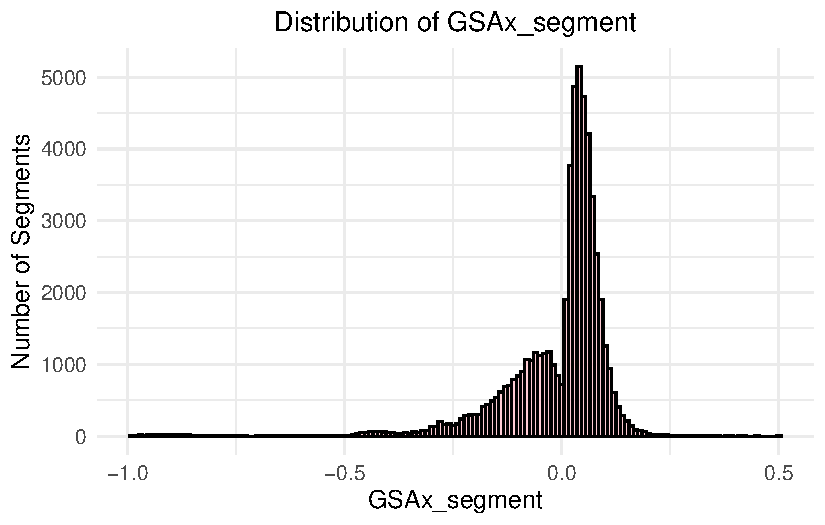
\includegraphics[width=0.67\textwidth,height=\textheight]{paper_files/figure-pdf/fig-1-1.pdf}

}

\caption{\label{fig-1}Distribution of GSAx\_segment}

\end{figure}%

From Figure~\ref{fig-1}, the distribution sharply peaks near 0, with a
long tail extending toward both positive and negative extremes; this
indicates most time segments exhibit performance close to expected
levels, with occasional outliers where goaltenders significantly
underperform or overperform. The distribution's longer negative tail
reflects the occasional high-impact errors (e.g., letting in unexpected
goals) that skews \texttt{GSAx\_segment} in short time frames.

\subsubsection{Predictor variables}\label{predictor-variables}

\paragraph{Game state predictors: Home vs Away, Regular Season vs
Playoffs}\label{game-state-predictors-home-vs-away-regular-season-vs-playoffs}

\texttt{isHomeTeam} is a binary variable equal to 1 if the goaltender is
playing at home, and 0 if playing away. This variable examines the
impact of home-ice advantage on performance, given that teams
historically perform better at home Bischof (2021).

\texttt{isPlayoffGame} is a binary variable equal to 1 for playoff games
and 0 for regular-season games. Playoff games are higher-stakes,
lower-scoring environments that may influence a goaltender's mindset,
workload, or performance Donchess (2022). By including this variable, we
assess whether this affects performance.

These game state variables are static for each segment, as segments
occur entirely within single games. Table~\ref{tbl-2} summarizes the
dataset's segments, categorized by the two predictors.

\begin{longtable}[]{@{}llr@{}}

\caption{\label{tbl-2}Count of segments by game state}

\tabularnewline

\toprule\noalign{}
Is Home Team & Is Playoff Game & Count \\
\midrule\noalign{}
\endhead
\bottomrule\noalign{}
\endlastfoot
0 & 0 & 26436 \\
1 & 0 & 26517 \\
0 & 1 & 1681 \\
1 & 1 & 1686 \\

\end{longtable}

As expected, the dataset primarily contains regular-season games.
Additionally, the \texttt{GSAx\_segments} for home and away games are
similar, as each game involves one goalie playing at home and another
playing away; discrepancies are attributable to infrequent goaltender
substitutions.

\paragraph{In-game performance and workload predictors: period, score,
shots faced, shots in last 3 minutes, performance so
far}\label{sec-period}

\texttt{period} is a categorical variable representing the period the
segment takes place in, created by splitting the game into 20-minute
intervals. Note that since segments are 10 minutes and almost all
periods are 20 minutes, every segment will take place within one period.
The only exception is regular season 5 minute overtime periods, but
these are guaranteed to be the game's final period, so it still holds
true that no segment overlaps periods.

We analyze if the period has any effect on goaltender performance,
choosing to represent periods categorically to capture unique
performance differences in each period without assuming a linear
progression. In Table~\ref{tbl-3} and Table~\ref{tbl-4} we see segments
that fall in each period for regular season and playoff games.

\begin{longtable}[]{@{}lr@{}}

\caption{\label{tbl-3}Segment breakdown for regular season periods}

\tabularnewline

\toprule\noalign{}
Period & Number of Segments \\
\midrule\noalign{}
\endhead
\bottomrule\noalign{}
\endlastfoot
1st Period & 17100 \\
2nd Period & 17194 \\
3rd Period & 17050 \\
Overtime & 1609 \\

\end{longtable}

Predictably, segments are similar across the first 3 periods. We can
infer that roughly 10\% of games require the extra 5-minute overtime
period.

\begin{longtable}[]{@{}lr@{}}

\caption{\label{tbl-4}Segment breakdown for playoff periods}

\tabularnewline

\toprule\noalign{}
Period & Number of Segments \\
\midrule\noalign{}
\endhead
\bottomrule\noalign{}
\endlastfoot
1st Period & 1064 \\
2nd Period & 1076 \\
3rd Period & 1056 \\
Overtime & 138 \\
2nd OT or later & 33 \\

\end{longtable}

Periods are similar for playoff games, with the difference being that
overtime periods are the same length as regular periods, and additional
overtime periods are required if there is no scoring. Roughly 13\% of
games require overtime.

\begin{itemize}
\tightlist
\item
  \texttt{goalieTeamScoreDifferential} represents the average
  differential of the game score over the course of the 10 minute
  segment. It is positive if the goaltender's team is leading, 0 if the
  game is tied, and negative if the goaltender's team is trailing; this
  allows us to analyze whether goaltenders perform better when their
  team is winning or losing, or depending on how close the game is.
  Decimal values reflect score changes within the segment.
\end{itemize}

\begin{longtable}[]{@{}lr@{}}

\caption{\label{tbl-5}Summary of segments by goaltender team score
differential}

\tabularnewline

\toprule\noalign{}
Summary Statistic & Goalie Team Score Diff. \\
\midrule\noalign{}
\endhead
\bottomrule\noalign{}
\endlastfoot
Min & -9.5 \\
1st Quantile.25\% & -0.9 \\
Median & 0.0 \\
Mean & 0.0 \\
3rd Quantile.75\% & 1.0 \\
Max & 9.5 \\
Standard Deviation & 1.6 \\

\end{longtable}

Table~\ref{tbl-5} shows this stat is symmetrical, as every non-tied
segment has a winning and losing goalie. Both the median and mean are 0,
representing tied segments. The median and mean is 0, representing
segments where the game is tied. Due to its symmetry, we can better
visualize the \texttt{goalieTeamScoreDifferential} distribution by
taking the absolute value in Figure~\ref{fig-2}.

\begin{figure}

\centering{

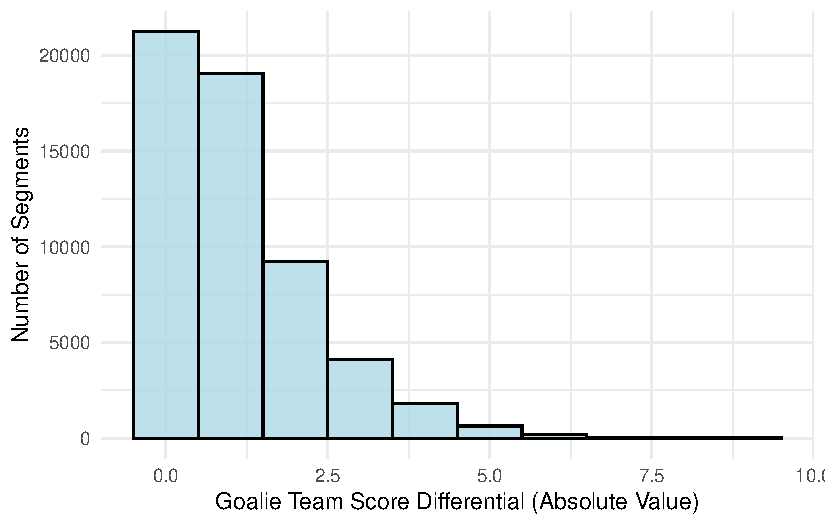
\includegraphics[width=0.67\textwidth,height=\textheight]{paper_files/figure-pdf/fig-2-1.pdf}

}

\caption{\label{fig-2}Distribution of the absolute value of the score
differential in segments.}

\end{figure}%

Most segments occur when the game is tied, and the number of segments
decreases exponentially with an increase in score differential. Segments
with a larger differential are rarer, as games tend to remain close in
score.

To analyze for winning and losing game states without the symmetry
effect, we can look at the distribution for an individual goaltender
such as Vancouver's Thatcher Demko. From Figure~\ref{fig-3}, many
segments were tied throughout, and he spent slightly more time with his
team winning. Most segments have unchanging score differentials,
categorized by the integer average.

\begin{figure}

\centering{

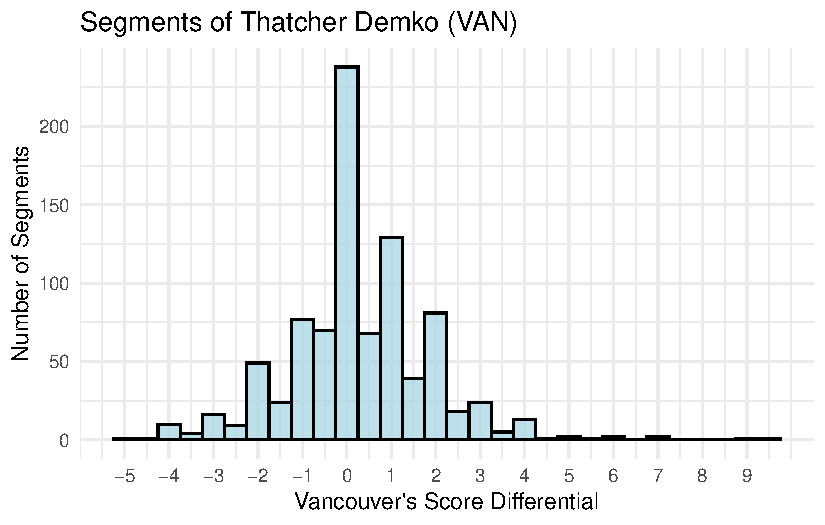
\includegraphics[width=0.67\textwidth,height=\textheight]{paper_files/figure-pdf/fig-3-1.pdf}

}

\caption{\label{fig-3}Distribution of the score differential for
segments of goaltender Thatcher Demko.}

\end{figure}%

\begin{itemize}
\tightlist
\item
  \texttt{shots\_faced} represents the cumulative number of shots a
  goaltender has faced in the game prior to each shot in the segment,
  averaged over each shot. This gives a measure of the goaltender's
  prior workload; we analyze how it influences the goaltender's ability
  to stop subsequent shots.
\end{itemize}

\begin{longtable}[]{@{}lr@{}}

\caption{\label{tbl-6}Summary of segments by shots faced}

\tabularnewline

\toprule\noalign{}
Summary Statistic & Shots Faced \\
\midrule\noalign{}
\endhead
\bottomrule\noalign{}
\endlastfoot
Min & 0 \\
1st Quantile.25\% & 6 \\
Median & 14 \\
Mean & 15 \\
3rd Quantile.75\% & 22 \\
Max & 78 \\
Standard Deviation & 10 \\

\end{longtable}

From Table~\ref{tbl-6}, the mean of 15 indicates that a goaltender has
faced 15 prior shots across the average segment. The maximum prior
workload for a segment was 78 shots.

\begin{figure}

\centering{

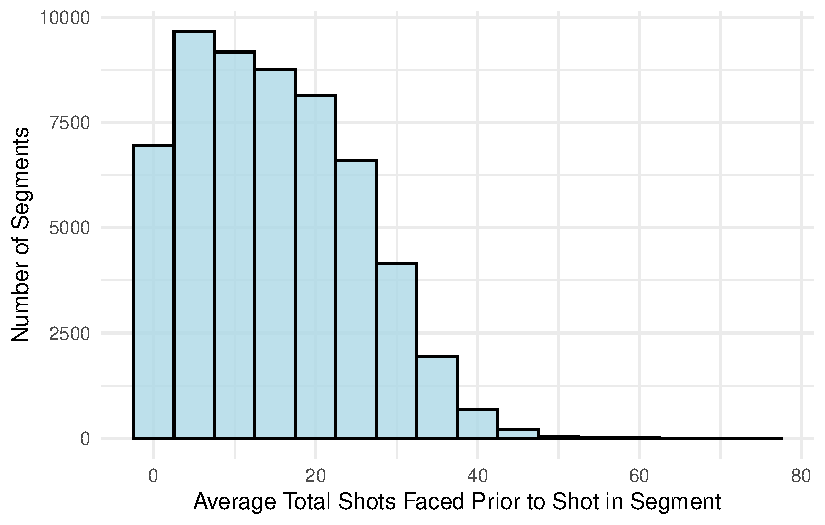
\includegraphics[width=0.67\textwidth,height=\textheight]{paper_files/figure-pdf/fig-4-1.pdf}

}

\caption{\label{fig-4}Distribution of shots faced so far, averaged
across shots in segment.}

\end{figure}%

We see in Figure~\ref{fig-4} that the distribution of
\texttt{shots\_faced} is close to uniform for values between 0-25.
Beyond 20 shots, the number of segments decreases exponentially,
reflecting that fewer games reach very high shot counts.

\begin{itemize}
\tightlist
\item
  \texttt{shotslast3min} finds the shots the goaltender has faced in the
  3 minutes prior to each shot in the segment, then takes the average
  across all shots in the segment. Note this is not equivalent to the
  shots faced in the 3 minutes prior to the segment; it is a dynamic
  value that can vary for each shot in the segment. By measuring this
  value, we evaluate whether facing many shots in quick succession can
  improve performance by keeping the goaltender ``in rhythm'' or more
  alert, or decrease performance by increasing pressure on the
  goaltender.
\end{itemize}

\begin{longtable}[]{@{}lr@{}}

\caption{\label{tbl-7}Summary of segments by the average shots faced in
the last 3 minutes, across segment shots.}

\tabularnewline

\toprule\noalign{}
Summary Statistic & ShotsLast3min \\
\midrule\noalign{}
\endhead
\bottomrule\noalign{}
\endlastfoot
Min & 0.0 \\
1st Quantile.25\% & 0.7 \\
Median & 1.2 \\
Mean & 1.3 \\
3rd Quantile.75\% & 1.8 \\
Max & 9.0 \\
Standard Deviation & 0.8 \\

\end{longtable}

From Table~\ref{tbl-7} and Figure~\ref{fig-5}, segments are roughly
normally distributed with a mean of 1.3, meaning a goaltender saw
\textasciitilde1.3 shots in the 3 minutes prior to every shot in an
average segment. Segments ranged from those with no shots in the
preceding 3 minutes to segments where the goaltender saw an average of 9
shots in the last 3 minutes.

\begin{figure}

\centering{

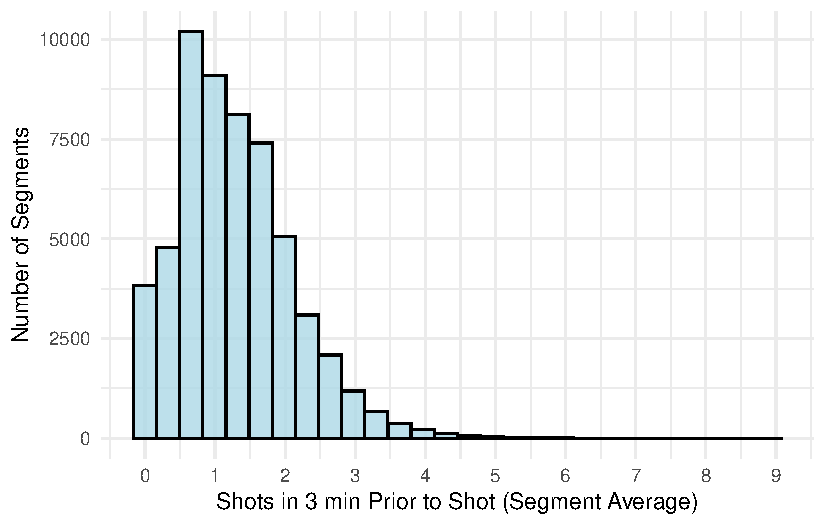
\includegraphics[width=0.67\textwidth,height=\textheight]{paper_files/figure-pdf/fig-5-1.pdf}

}

\caption{\label{fig-5}Distribution of segments depending on average
shots seen in the last 3 minutes averaged across the segment.}

\end{figure}%

\begin{itemize}
\tightlist
\item
  \texttt{GSAx\_so\_far} is the cumulative GSAx of a goaltender up to
  the current point in the game, prior to the shots in the segment. This
  variable captures how well a goaltender has performed relative to
  expectation throughout the game up to the current moment, enabling
  exploration of whether strong performance early in a game carries over
  into later segments, and vice versa.
\end{itemize}

\begin{longtable}[]{@{}lr@{}}

\caption{\label{tbl-8}Summary of segments by accumulated GSAx prior to
segment.}

\tabularnewline

\toprule\noalign{}
Summary Statistic & GSAx so far \\
\midrule\noalign{}
\endhead
\bottomrule\noalign{}
\endlastfoot
Min & -5.98 \\
1st Quantile.25\% & -0.44 \\
Median & 0.12 \\
Mean & 0.10 \\
3rd Quantile.75\% & 0.64 \\
Max & 6.06 \\
Standard Deviation & 1.01 \\

\end{longtable}

In Table~\ref{tbl-8}, the median 0.12 and mean 0.1 suggest that
goaltender performance prior to segments is generally close to
expectations, with slight overperformance common. In Figure~\ref{fig-6}
the distribution is approximately normal and centered near 0; the range
(-5.98 to 6.06) and standard deviation 1.01 indicate considerable
variability in in-game performance.

\begin{figure}

\centering{

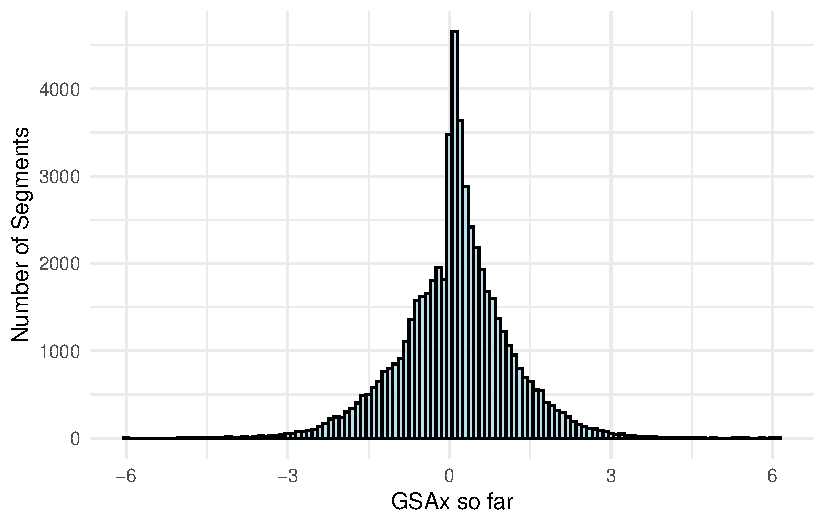
\includegraphics[width=0.67\textwidth,height=\textheight]{paper_files/figure-pdf/fig-6-1.pdf}

}

\caption{\label{fig-6}Distribution of segments based on the goaltender's
accumulated GSAx prior to segment.}

\end{figure}%

\paragraph{Recent performance predictors: Last game and last 5
games}\label{recent-performance-predictors-last-game-and-last-5-games}

\begin{itemize}
\tightlist
\item
  \texttt{last\_game\_GSAx} represents the goaltender's performance in
  the previous game, measured with the cumulative GSAx.
\item
  \texttt{last\_5\_avg\_GSAx} representing the goaltender's performance
  in the previous 5 games, measured with average cumulative GSAx.
\end{itemize}

With these, we can see if the previous performance or stretch of
performances carries over to the next goaltender performance.

\begin{longtable}[]{@{}lr@{}}

\caption{\label{tbl-9}Summary of segments by goaltender GSAx in the
previous game.}

\tabularnewline

\toprule\noalign{}
Summary Statistic & Last game GSAx \\
\midrule\noalign{}
\endhead
\bottomrule\noalign{}
\endlastfoot
Min & -5.99 \\
1st Quantile.25\% & -0.99 \\
Median & 0.12 \\
Mean & 0.06 \\
3rd Quantile.75\% & 1.13 \\
Max & 6.99 \\
Standard Deviation & 1.59 \\

\end{longtable}

\begin{figure}

\centering{

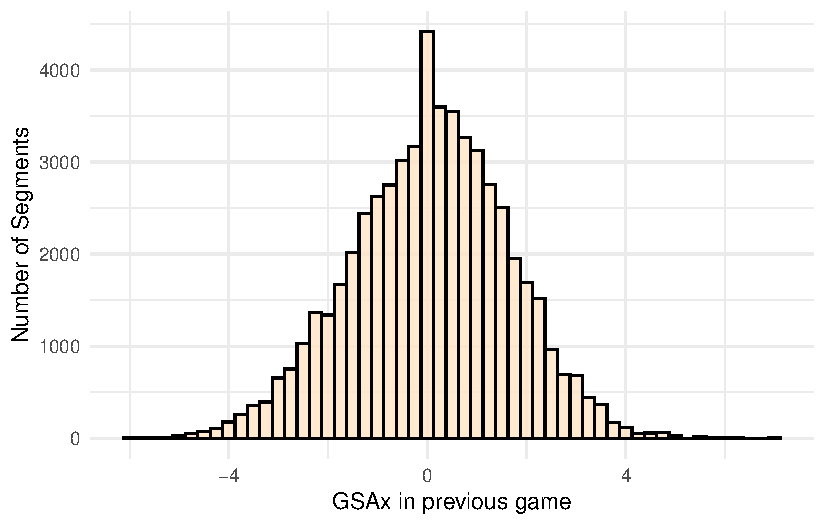
\includegraphics[width=0.67\textwidth,height=\textheight]{paper_files/figure-pdf/fig-7-1.pdf}

}

\caption{\label{fig-7}Distribution of segments based on the goaltender's
previous game GSAx.}

\end{figure}%

From Figure~\ref{fig-7}, we observe a roughly normal distribution
centered near 0, which aligns with expectations. The mean of 0.06 in
Table~\ref{tbl-9} may reflect a selection effect, as goaltenders with
particularly poor performances in their previous games may not play in
the following game, skewing the distribution slightly toward positive
values.

From Figure~\ref{fig-8}, when we increase the prior performance sample
to 5 games, the tails are shorter, with average GSAx falling mostly
between -2 and 2. The lower standard deviation in Table~\ref{tbl-10}
confirms this. Other variable features are similar to
\texttt{last\_game\_GSAx}.

\begin{longtable}[]{@{}lr@{}}

\caption{\label{tbl-10}Summary of segments by average goaltender GSAx in
the previous 5 games.}

\tabularnewline

\toprule\noalign{}
Summary Statistic & Last 5 Average GSAx \\
\midrule\noalign{}
\endhead
\bottomrule\noalign{}
\endlastfoot
Min & -5.99 \\
1st Quantile.25\% & -0.43 \\
Median & 0.06 \\
Mean & 0.06 \\
3rd Quantile.75\% & 0.55 \\
Max & 3.60 \\
Standard Deviation & 0.76 \\

\end{longtable}

\begin{figure}

\centering{

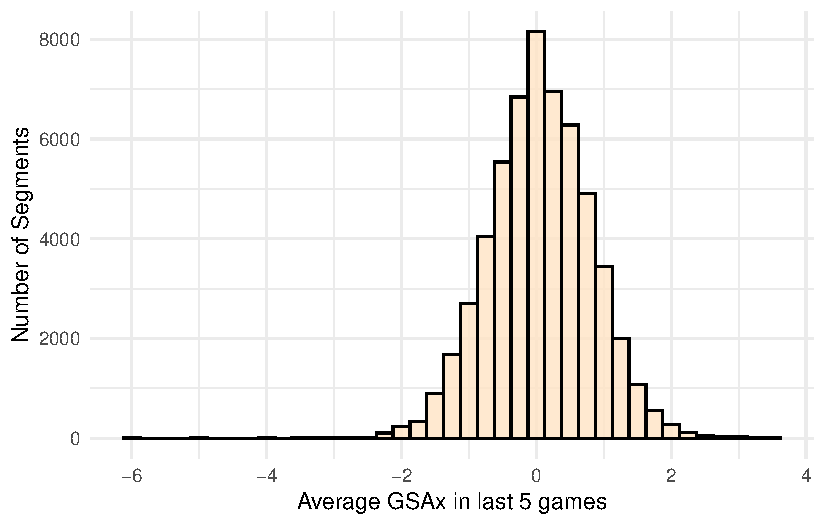
\includegraphics[width=0.67\textwidth,height=\textheight]{paper_files/figure-pdf/fig-8-1.pdf}

}

\caption{\label{fig-8}Distribution of segments based on the average GSAx
of the goaltender's previous 5 games.}

\end{figure}%

\newpage

\section{Model}\label{sec-model}

Using the statistical programming software R (R Core Team 2023) as well
as packages (Wickham et al. 2019), (Arel-Bundock 2022) and (Kuhn and Max
2008), we develop a linear regression model with \texttt{GSAx\_segment}
as the response variable and our outlined factors as predictor
variables. The objective of this model is to identify which predictors
significantly influence goaltender performance, using p-values to assess
significance and coefficients to evaluate the magnitude of their
effects.

Alternative modeling approaches were considered, such as using
shot-level or game-cumulative GSAx as the response variable. These
approaches analyze different levels of granularity; we chose the
segment-based model as it is detailed and interpretable. It focuses on
how external factors shape performance without introducing excessive
uncertainty or overly broadening the scope of analysis. This aligns with
the goal of understanding the predictors' effect on the response rather
than creating a highly predictive model.

Background details and diagnostics are included in
Appendix~\ref{sec-model-details}

\subsection{Model}\label{model}

\begin{align}
\text{GSAx\_segment}_i &= \beta_0 
+ \beta_1 \times \text{isHomeTeam}_i \\
& \quad + \beta_2 \times \text{isPlayoffGame}_i \\
& \quad + \beta_3 \times \text{period2nd Period}_i \\
& \quad + \beta_4 \times \text{period3rd Period}_i \\
& \quad + \beta_5 \times \text{periodOvertime}_i \\
& \quad + \beta_6 \times \text{period2nd OT or later}_i \\
& \quad + \beta_7 \times \text{goalieTeamScoreDifferential}_i \\
& \quad + \beta_8 \times \text{shots\_faced}_i \\
& \quad + \beta_9 \times \text{shotslast3min}_i \\
& \quad + \beta_{10} \times \text{GSAx\_so\_far}_i \\
& \quad + \beta_{11} \times \text{last\_game\_GSAx}_i \\
& \quad + \beta_{12} \times \text{last\_5\_avg\_GSAx}_i \\
& \quad + \beta_{13} \times (\text{isHomeTeam}_i \times \text{isPlayoffGame}_i) \\
& \quad + \beta_{14} \times (\text{goalieTeamScoreDifferential}_i \times \text{shotslast3min}_i) \\
& \quad + \beta_{15} \times (\text{goalieTeamScoreDifferential}_i \times \text{shots\_faced}_i) \\
& \quad + \beta_{16} \times (\text{GSAx\_so\_far}_i \times \text{shotslast3min}_i)
\end{align}

\begin{itemize}
\item
  \(\beta_0\): The intercept of the model, representing the expected
  value of \texttt{GSAx\_segment} when all predictors are set to zero
  (i.e., when the game is neither a home game nor a playoff game, the
  score differential is zero, and no shots have been faced in the last
  three minutes, etc.).
\item
  \(\beta_1\): The coefficient representing the change in
  \texttt{GSAx\_segment} when the game is a home game (as indicated by
  \texttt{isHomeTeam\ =\ 1}), compared to when the game is an away game,
  holding all other variables constant.
\item
  \(\beta_2\): The coefficient representing the change in
  \texttt{GSAx\_segment} when the game is a playoff game
  (\texttt{isPlayoffGame\ =\ 1}), compared to when it is a regular
  season game, holding all other variables constant.
\item
  \(\beta_3, \beta_4, \beta_5, \beta_6\): The coefficients representing
  the change in \texttt{GSAx\_segment} compared to the baseline 1st
  period, depending on if the game is in the 2nd, 3rd, OT, or extra OT
  periods respectively, holding all other variables constant. As
  discussed in Section~\ref{sec-period}, \texttt{period} is categorical
  to avoid assuming a linear progression.
\item
  \(\beta_7\): The coefficient representing the change in
  \texttt{GSAx\_segment} for a one-unit increase in the
  \texttt{goalieTeamScoreDifferential}, holding all other variables
  constant. This variable measures the score difference between the
  goaltender's team and the opponent, reflecting the impact of game
  context on goaltender performance.
\item
  \(\beta_8\): The coefficient representing the change in
  \texttt{GSAx\_segment} for a one-unit increase in
  \texttt{shots\_faced} by the goaltender during the game, holding all
  other predictors constant. This represents how goaltender performance
  changes with an increased workload.
\item
  \(\beta_9\): The coefficient representing the change in
  \texttt{GSAx\_segment} for a one-unit increase in the number of
  \texttt{shotslast3min}, the average count of shots faced in the last 3
  minutes, holding all other predictors constant. This quantifies how
  recent shot activity affects the goaltender's performance.
\item
  \(\beta_{10}\): The coefficient representing the change in
  \texttt{GSAx\_segment} for a one-unit increase in
  \texttt{GSAx\_so\_far}, the prior cumulative performance of the
  goaltender, holding all other predictors constant. This accounts for
  how a goaltender's in-game performance thus far influences current
  performance.
\item
  \(\beta_{11}\): The coefficient representing the change in
  \texttt{GSAx\_segment} when the goaltender's performance in the
  previous game (\texttt{last\_game\_GSAx}) increases by one GSAx,
  holding all other predictors constant. This captures the effect of
  previous game performance trend on current performance.
\item
  \(\beta_{12}\): The coefficient representing the change in
  \texttt{GSAx\_segment} when the average performance over the last five
  games (\texttt{last\_5\_avg\_GSAx}) increases by one GSAx, holding all
  other predictors constant. This captures the effect of the
  goaltender's longer-term performance trend on current performance.
\item
  \(\beta_{13}\): The coefficient representing the change in
  \texttt{GSAx\_segment} due to the interaction between being a home
  game (\texttt{isHomeTeam}) and a playoff game
  (\texttt{isPlayoffGame}). This accounts for how home-ice advantage may
  differ in high-stakes playoff games and how this combination
  influences goaltender performance.
\item
  \(\beta_{14}\): The coefficient representing the change in
  \texttt{GSAx\_segment} due to the interaction between
  \texttt{goalieTeamScoreDifferential} and \texttt{shotslast3min},
  recognizing that the goaltenders may be affected differently by recent
  shot activity depending on the game score.
\item
  \(\beta_{15}\): The coefficient representing the change in
  \texttt{GSAx\_segment} due to the interaction between
  \texttt{goalieTeamScoreDifferential} and \texttt{shots\_faced}.
  recognizing that the goaltenders may be affected differently by a high
  workload depending on the game score.
\item
  \(\beta_{16}\): The coefficient representing the change in
  \texttt{GSAx\_segment} due to the interaction between
  \texttt{GSAx\_so\_far} and \texttt{shotslast3min}, accounting for how
  a goaltender's prior performance and recent shot activity jointly
  impact their current performance.
\end{itemize}

\subsection{Assumptions and
validation}\label{assumptions-and-validation}

The model assumes no systematic relationship between the residuals and
the fitted values of the response variable, or between residuals and any
predictor. This ensures that the unexplained variance is random and does
not display patterns that might indicate unaddressed non-linear
relationships. We assess these assumptions using residuals vs.~fitted
values plots.

The model also assumes a linear relationship between the predictors and
the response variable GSAx\_segment. This means the effect of each
predictor on GSAx\_segment is additive and constant. Residual plots are
used to evaluate whether the linearity assumption holds.

Additionally, the model assumes that the residuals are normally
distributed, independent, and have constant variance (homoscedasticity).
If these assumptions are violated, the model's estimates may be biased
or invalid. We check these with a normal QQ plot.

We mentioned earlier in Section~\ref{sec-variables} that we need to
check for multicollinearity. Predictors should not be highly correlated,
as this can lead to unstable estimates and inflate standard errors. We
used Generalized Variance Inflation Factor (GVIF) analysis to identify
potential multicollinearity issues.

To validate the model, we perform a train-test split (80/20). The model
is fit using the training set, and performance is evaluated on the test
set using the Mean Squared Error (MSE) and R-squared values. Since the
R-squared of the model on the training and testing set is similar, we
conclude that the model generalizes well and is not overfit.

Further details and graphs are included in
Appendix~\ref{sec-model-details}.

\subsection{Limitations}\label{limitations}

There are a few limitations to our model:

Due to lack of data, the model does not include all possible external
factors influencing goaltender performance. Some other possible factors
include such as team overall performance, team tactics, current health,
days of rest since last game, contract situation, or game-specific
psychological factors. These omissions could lead to lack of model
precision or biased estimates for included predictors.

We assume linearity for all predictor variables. While this simplifies
the model, it may not fully capture the complexities of goaltender
performance.

The model's response variable has flaws, as discussed in
Section~\ref{sec-responsevariable}.

The R-squared value indicates that only a small portion of variance in
\texttt{GSAx\_segment} is explained by the model, so the model cannot be
used to draw extremely strong conclusions about the relationships
between our predictors and \texttt{GSAx\_segment}.

\subsection{Appropriate use}\label{appropriate-use}

There are some contexts where the model is not appropriate for use:

The model may not be suitable when interactions or dynamics beyond those
included (e.g., omitted variables discussed above) significantly
influence performance.

The model is designed to estimate the effects of external factors on
goaltender over- or underperformance rather than to maximize predictive
accuracy. As such, it does not perform well when asked to precisely
predict the response \texttt{GSAx\_segment}.

\section{Results}\label{sec-results}

Our model regression coefficients and their associated standard errors
are summarized in Table~\ref{tbl-modelresults}.

\begin{table}

\caption{\label{tbl-modelresults}Coefficient values and their errors}

\centering{

\centering
\begin{tblr}[         %% tabularray outer open
]                     %% tabularray outer close
{                     %% tabularray inner open
colspec={Q[]Q[]},
column{1}={halign=l,},
column{2}={halign=c,},
}                     %% tabularray inner close
\toprule
& (1) \\ \midrule %% TinyTableHeader
(Intercept)                                 & \num{-0.010}  \\
& (\num{0.001}) \\
isHomeTeam                                  & \num{-0.003}  \\
& (\num{0.001}) \\
isPlayoffGame                               & \num{0.005}   \\
& (\num{0.003}) \\
goalieTeamScoreDifferential                 & \num{0.011}   \\
& (\num{0.001}) \\
shotslast3min                               & \num{0.009}   \\
& (\num{0.001}) \\
shots\_faced                               & \num{-0.001}  \\
& (\num{0.000}) \\
period2nd OT or later                       & \num{-0.013}  \\
& (\num{0.025}) \\
period2nd Period                            & \num{0.000}   \\
& (\num{0.002}) \\
period3rd Period                            & \num{0.013}   \\
& (\num{0.003}) \\
periodOvertime                              & \num{-0.092}  \\
& (\num{0.004}) \\
GSAx\_so\_far                             & \num{0.022}   \\
& (\num{0.001}) \\
last\_game\_GSAx                          & \num{0.000}   \\
& (\num{0.000}) \\
last\_5\_avg\_GSAx                       & \num{0.001}   \\
& (\num{0.001}) \\
isHomeTeam × isPlayoffGame                  & \num{-0.001}  \\
& (\num{0.005}) \\
goalieTeamScoreDifferential × shotslast3min & \num{0.001}   \\
& (\num{0.000}) \\
goalieTeamScoreDifferential × shots\_faced & \num{-0.001}  \\
& (\num{0.000}) \\
shotslast3min × GSAx\_so\_far             & \num{0.002}   \\
& (\num{0.001}) \\
\bottomrule
\end{tblr}

}

\end{table}%

\subsection{Coefficient
Interpretation}\label{coefficient-interpretation}

From the provided table of regression coefficients, we can draw the
conclusions about the model's results. Each coefficient represents the
magnitude of the effect of the corresponding variable or interaction
term on GSAx\_segment, holding other variables constant. The standard
error (in parentheses) allows us to determine if terms are significant;
if the coefficients are a standard error from 0, and have p-values above
a 0.05 significance level, they are likely insignificant.

\subsubsection{Significant terms}\label{significant-terms}

Binary/Categorical:

\begin{itemize}
\item
  \texttt{isHomeTeam}\strut \\
  Coefficient: \texttt{-0.003}\\
  Implication: Playing at home is associated with a slight decrease in
  \texttt{GSAx\_segment}, suggesting that goaltenders may slightly
  underperform at home.
\item
  \texttt{period3rd\ Period}\strut \\
  Coefficient: \texttt{0.013}\\
  Implication: Performance improves slightly in the 3rd period compared
  to the baseline 1st period.
\item
  \texttt{periodOvertime}\strut \\
  Coefficient: \texttt{-0.091}\\
  Implication: Goaltenders perform significantly worse during overtime
  compared to the baseline 1st period.
\end{itemize}

Continuous:

\begin{itemize}
\item
  \texttt{goalieTeamScoreDifferential}\strut \\
  Coefficient: \texttt{0.011}\\
  Implication: An increase in the score differential (goalie's team
  scores a goal) is associated with an increase in
  \texttt{GSAx\_segment}, indicating improved goaltender performance
  when leading.
\item
  \texttt{shotslast3min}\strut \\
  Coefficient: \texttt{0.009}\\
  Implication: Facing more shots in the last three minutes is associated
  with a better \texttt{GSAx\_segment}, suggesting that recent activity
  may keep the goaltender in a rhythm or alert.
\item
  \texttt{shots\_faced}\strut \\
  Coefficient: \texttt{-0.001}\\
  Implication: Each additional shot faced is associated with a small
  decrease in \texttt{GSAx\_segment}, suggesting that increased workload
  slightly reduces performance.
\item
  \texttt{GSAx\_so\_far}\strut \\
  Coefficient: \texttt{0.022}\\
  Implication: Better cumulative performance earlier in the game is
  associated with improved performance during the segment, indicating
  momentum or consistency.
\item
  \texttt{shotslast3min:GSAx\_so\_far}\strut \\
  Coefficient: \texttt{0.002}\\
  Implication: The interaction between recent activity (shots in the
  last three minutes) and cumulative performance
  (\texttt{GSAx\_so\_far}) suggests that recent activity amplifies the
  positive effects of prior performance.
\end{itemize}

Effect of continuous predictors on \texttt{GSAx\_segment}: for a
one-unit increase in each of the 5 continuous variables/interaction
terms above, \texttt{GSAx\_segment} changes by the magnitude of the
coefficient. For example, if the goalie's team were to score an extra
goal, \texttt{GSAx\_segment} would increase by 0.011.

Although the coefficients are small, they still have some significance.
For example, the 0.013 coefficient for period3rd Period can be
interpreted as a 1.3\% increase in goaltender performance in the 3rd
period compared to the 1st.

\subsubsection{Insignificant terms}\label{insignificant-terms}

The coefficients for these variables are likely to be 0, meaning the
effects of these variables on \texttt{GSAx\_segment} are not strong
enough to make conclusions:

\begin{itemize}
\tightlist
\item
  Intercept: The baseline value itself is not particularly meaningful
  since most predictors will not realistically be zero.
\item
  \texttt{isPlayoffGame}\strut \\
\item
  \texttt{period2nd\ OT\ or\ later}\strut \\
\item
  \texttt{period2nd\ Period}\strut \\
\item
  \texttt{last\_game\_GSAx}\strut \\
\item
  \texttt{last\_5\_avg\_GSAx}\strut \\
\item
  \texttt{isHomeTeam:isPlayoffGame}\strut \\
\item
  \texttt{goalieTeamScoreDifferential:shotslast3min}
\end{itemize}

\subsection{Effects of Significant
Terms}\label{effects-of-significant-terms}

To better visualize the effects of significant terms, here are how the
values of \texttt{GSAx\_segment} differ for each of our significant
terms.

\subsubsection{Home vs Away}\label{home-vs-away}

Table~\ref{tbl-homeaway} compares goaltender performance
\texttt{GSAx\_segment} between home and away games. The average
GSAx\_segment for away games is -0.0076, while for home games, it is
-0.0087. This small difference (-0.0012) is consistent with the model
findings, indicating that goaltenders perform slightly worse at home,
with a 0.12\% decrease in performance. This could be due to increased
pressure at home, although 0.12\% is a very small difference.

\begin{longtable}[]{@{}lrr@{}}

\caption{\label{tbl-homeaway}GSAx\_segment values for home and away}

\tabularnewline

\toprule\noalign{}
Goaltender Team & Count & Avg GSAx\_Segment \\
\midrule\noalign{}
\endhead
\bottomrule\noalign{}
\endlastfoot
Away & 28117 & -0.0075587 \\
Home & 28203 & -0.0087676 \\

\end{longtable}

\subsubsection{Goalie Team Score
Differential}\label{goalie-team-score-differential}

\begin{longtable}[]{@{}crr@{}}

\caption{\label{tbl-scorediff}GSAx\_segment values by score
differential}

\tabularnewline

\toprule\noalign{}
Score Differential & Segments & Avg GSAx of Segment \\
\midrule\noalign{}
\endhead
\bottomrule\noalign{}
\endlastfoot
4+ & 1461 & 0.0159524 \\
3 & 2054 & 0.0177675 \\
2 & 5214 & 0.0112033 \\
1 & 9567 & 0.0117394 \\
0 & 21234 & -0.0091289 \\
-1 & 8840 & -0.0255358 \\
-2 & 4660 & -0.0336153 \\
-3 & 1886 & -0.0323749 \\
-4+ & 1404 & -0.0377781 \\

\end{longtable}

Table~\ref{tbl-scorediff} summarizes \texttt{GSAx\_segment} values based
on the game score, represented as the score differential of the goalie's
team. As the goaltender's team gains an additional goal, the average
\texttt{GSAx\_segment} improves, from being negative when the
goaltending team is trailing to positive when the team is ahead. The
data reveals a trend where goaltenders perform better as their team
increases their lead, likely due to reduced pressure or easier defensive
situations. Conversely, performance decreases when the team is trailing,
potentially reflecting higher-pressure situations or increased shot
difficulty.

\subsubsection{Shots faced in last 3
minutes}\label{shots-faced-in-last-3-minutes}

\begin{longtable}[]{@{}crr@{}}

\caption{\label{tbl-last3}GSAx\_segment values versus shots faced in
last 3 minutes}

\tabularnewline

\toprule\noalign{}
Avg. Shots in last 3 min & Segments & Avg GSAx of Segment \\
\midrule\noalign{}
\endhead
\bottomrule\noalign{}
\endlastfoot
0 & 11710 & -0.0286755 \\
1 & 24307 & -0.0062646 \\
2 & 15969 & -0.0008660 \\
3 & 3525 & 0.0094621 \\
4 & 703 & 0.0088892 \\
5+ & 106 & 0.0234829 \\

\end{longtable}

Table~\ref{tbl-last3} examines how recent shot activity influences
goaltender performance. Segments with zero shot activity have the lowest
average \texttt{GSAx\_segment} at -0.029; this steadily increases until
we reach segments with five or more shots, which have the highest
average of 0.024. This trend suggests that goaltenders perform better
when actively engaged, possibly due to improved focus or rhythm.
Conversely, performance decreases when goaltenders are inactive for
extended periods.

\begin{figure}

\centering{

\begin{longtable*}[]{@{}crr@{}}
\toprule\noalign{}
Shots Faced So Far & Segments & Avg GSAx of Segment \\
\midrule\noalign{}
\endhead
\bottomrule\noalign{}
\endlastfoot
0-5 & 12260 & -0.0038470 \\
5-10 & 9116 & -0.0048480 \\
10-15 & 8887 & -0.0073134 \\
15-20 & 8564 & -0.0074205 \\
20-25 & 7527 & -0.0091401 \\
25-30 & 5317 & -0.0132248 \\
30-35 & 2965 & -0.0197011 \\
35+ & 1684 & -0.0251613 \\
\end{longtable*}

}

\caption{\label{fig-shots}GSAx\_segment values versus cumulative shots
faced}

\end{figure}%

Figure~\ref{fig-shots} examines the relationship between the total
number of shots faced by a goaltender so far in a game and the
corresponding \texttt{GSAx\_segment}. The data show a clear downward
trend in performance as the cumulative number of shots faced increases.
Segments where the goaltender has faced 0--5 shots have the highest
average \texttt{GSAx\_segment} of -0.003, and this decreases until we
reach segments with 35 or more shots, with average
\texttt{GSAx\_segment} -0.025.

This trend suggests that as goaltenders face more shots over the course
of a game, their performance tends to decline. This may be due to
physical fatigue or mental strain as the game prorgresses. Notably, the
decline in performance accelerates beyond 25 shots, indicating that
heavy workloads can have a pronounced negative impact on
\texttt{GSAx\_segment}.

\begin{figure}

\centering{

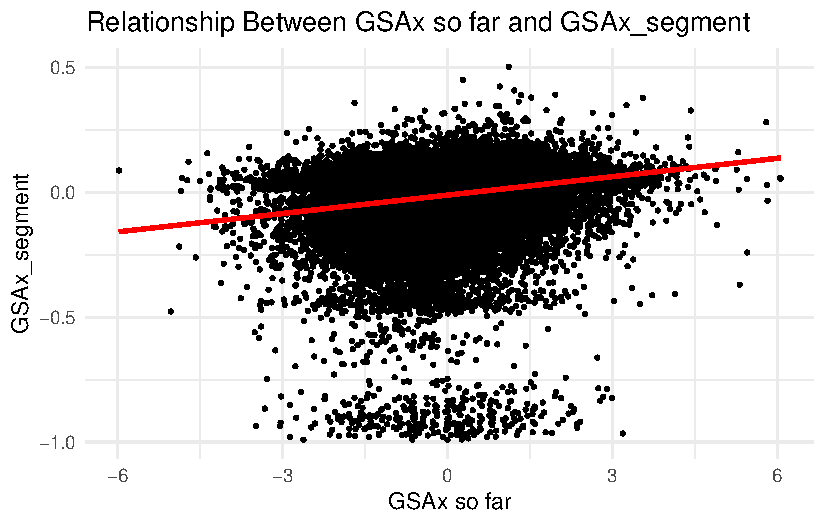
\includegraphics{paper_files/figure-pdf/fig-sofar-1.pdf}

}

\caption{\label{fig-sofar}Scatterplot of GSAx\_segment values versus
GSAx\_so\_far}

\end{figure}%

Figure~\ref{fig-sofar} shows the relationship between a goaltender's
cumulative performance up to a given segment, measured by
\texttt{GSAx\_so\_far}, and their performance during that segment
\texttt{GSAx\_segment}. The positive slope of the trend line indicates
that better cumulative performance is associated with better segment
performance. This suggests a momentum effect, where goaltenders who
perform well earlier in the game are more likely to continue performing
well.

However, the spread of residuals shows significant variability in
segment performance, showing that \texttt{GSAx\_so\_far} is still far
from fully explaining segment performance, and the relationship between
the two is relatively weak. This aligns with the model finding that
\texttt{GSAx\_so\_far} has a significant but modest effect size.

\section{Discussion}\label{sec-discussion}

\subsection{Significant Predictors of Goaltender
Overperformance}\label{significant-predictors-of-goaltender-overperformance}

The analysis identifies several significant predictors that shape
goaltender performance, as measured by goals saved above expected over
10 minute segments. Among these, score differential shows that
performance improves as the goaltender's team takes a lead, reflecting
reduced pressure or fewer high-quality scoring chances when leading.
This result highlights the importance of game context in shaping
outcomes, as trailing teams may expose their goaltenders to more
challenging scenarios, and winning teams may put extra effort into
defending their goaltender.

Recent shot activity also plays a meaningful role, with increased
engagement in the minutes preceding a segment positively affecting
performance. This suggests that consistent involvement helps goaltenders
maintain focus and rhythm. Conversely, the cumulative number of shots
faced in a game negatively impacts performance, illustrating the toll of
sustained workloads and fatigue.

The sum of in-game GSAx prior to segments, a measure of cumulative
performance within the game, has a positive relationship with segment
performance, suggesting momentum or consistency. Goaltenders who perform
well earlier in the game are more likely to sustain that level of
performance later. The interaction between this variable and recent shot
activity underscores this trend, indicating that recent activity
enhances the positive effects of prior performance.

\subsection{Insignificant Predictors and their
Implications}\label{insignificant-predictors-and-their-implications}

Not all factors examined in the model significantly influenced
goaltender overperformance. Neither recent performance metrics, such as
goaltender overperformance in the previous or past 5 games, nor broader
game state variables like home/away or playoff status showed a
meaningful relationship with segment performance. These results suggest
that external situational factors within the game have a stronger impact
on goaltender outcomes than historical trends or the context surrounding
the game.

The lack of influence from recent performance metrics challenges the
popular notion of ``hot streaks'' among goaltenders. Similarly, the
negative effect of playing at home implies that home-ice advantage has
little bearing on individual goaltending performance, even if it is a
factor in overall team success. These findings reveal that in-game
dynamics are more likely to explain performance variability.

\subsection{Weaknesses and next steps}\label{weaknesses-and-next-steps}

As discussed, the analysis model has several limitations. First, the
relatively low predictive power indicates that many unmeasured variables
influence overperformance. Incorporating elements measuring factors such
as team overall performance, team tactics, current health, days of rest
since last game, contract situation, or game-specific psychological
factors in future models could enhance the explanatory power of the
analysis. New datasets could also help; for example, puck and player
tracking data would greatly supplement traditional event data, providing
in-game context that is currently unaccounted for.

The assumption of linear relationships between predictors and the
performance simplifies complex dynamics. For instance, the relationship
between workload and performance may follow a non-linear pattern, with
sharp declines after a certain threshold. Non-linear models or machine
learning approaches could address these complexities more effectively.
We could also create complex models combining segment-level data with
shot-level or game-level analysis, particularly during critical moments
in games.

Future work could also validate these findings across different leagues,
and levels of play. The NHL represents the best of the best and all of
its goaltenders are of elite skill level; it would be informative to see
what trends develop when analyzing data of lesser professionals or even
amateurs. Expanding the scope to include more holistic groups would
contribute to a more detailed understanding of what drives goaltender
performance under varying conditions.

\section{Extras}\label{extras}

A datasheet for the dataset is found in Gebru et al. (2018).

\newpage

\appendix

\section*{Appendix}\label{appendix}
\addcontentsline{toc}{section}{Appendix}

\section{Datasheet}\label{sec-datasheet}

\section{Surveys, sampling, and observational
data}\label{surveys-sampling-and-observational-data}

todo: copy this from google doc/form, fix residual plots code

\section{Data cleaning and preparation}\label{sec-appendix-a}

To clean the data, we first drop erroneous entries - shots with NA
values for goaltender name \texttt{goalieNameForShot}, boolean variable
\texttt{goal}, or identifier \texttt{game\_id}. We remove shots taken on
an empty net from when the goaltender was substituted for an extra
skater. In addition, we transform team variables categorized by
\texttt{home} or \texttt{away} team to the goalie's team or shooting
team, depending on which team is taking the shot.

We calculate variables required for our analysis model: Goals Saved
Above Expected (\texttt{GSAx}) for each shot is obtained by subtracting
the expected goal value of the shot \texttt{xGoal} from boolean value
\texttt{goal}. \texttt{xGoal} is modelled by Moneypuck based on many
other shot variables Tanner (2024).

\texttt{period}, which is categorical, is obtained based on the
\texttt{time} in seconds elapsed. Goaltender-specific variables such as
\texttt{shots\_faced}, \texttt{shotslast3min} and \texttt{GSAx\_so\_far}
are obtained by counting shots and their associated GSAx.

Recent performance variables \texttt{last\_game\_GSAx} and
\texttt{last\_5\_avg\_GSAx} are calculated by first finding the current
game's total \texttt{GSAx} and average of the last 5 games,
respectively, and then shifting this data to the next game. We imputate
the NA values for \texttt{last\_game\_GSAx} and
\texttt{last\_5\_avg\_GSAx} (occurs for the goaltender's first game) by
assigning them to the median of the goalie's \texttt{last\_game\_GSAx}
and \texttt{last\_5\_avg\_GSAx} for the season.

Prior to modelling, we create 10-minute time segments based on
\texttt{time}, group all shots by segments, and average all of their
variables (both predictors and response) across the segment.

\section{Data manipulation details}\label{data-manipulation-details}

Data was cleaned using R Core Team (2023) and packages Richardson et al.
(2024), Wickham et al. (2019), Zeileis and Grothendieck (2005). Data was
tested and analyzed with Wickham (2011), Kuhn and Max (2008), and Xie
(2014). Data visualizations were created with Zhu (2021).

\section{Model details}\label{sec-model-details}

\subsubsection{Checking Residual vs Fitted
Values}\label{checking-residual-vs-fitted-values}

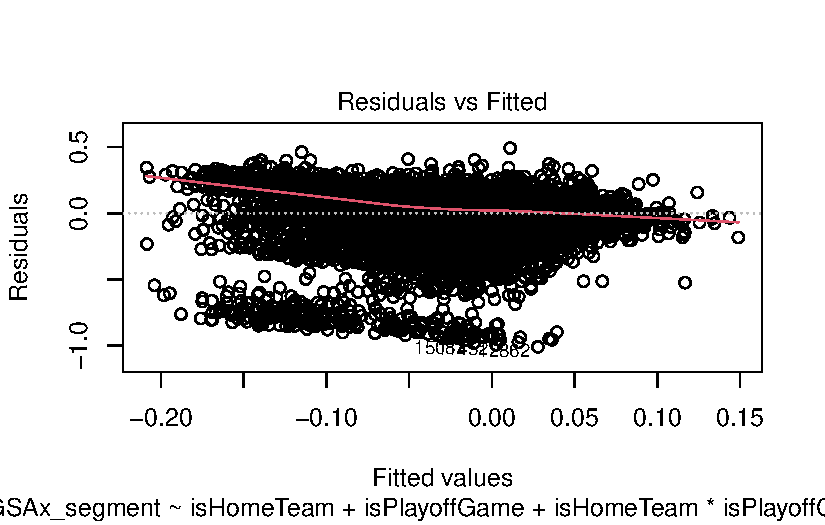
\includegraphics[width=0.5\textwidth,height=\textheight]{paper_files/figure-pdf/unnamed-chunk-27-1.pdf}

\subsubsection{Checking relationship between predictors and
residuals}\label{checking-relationship-between-predictors-and-residuals}

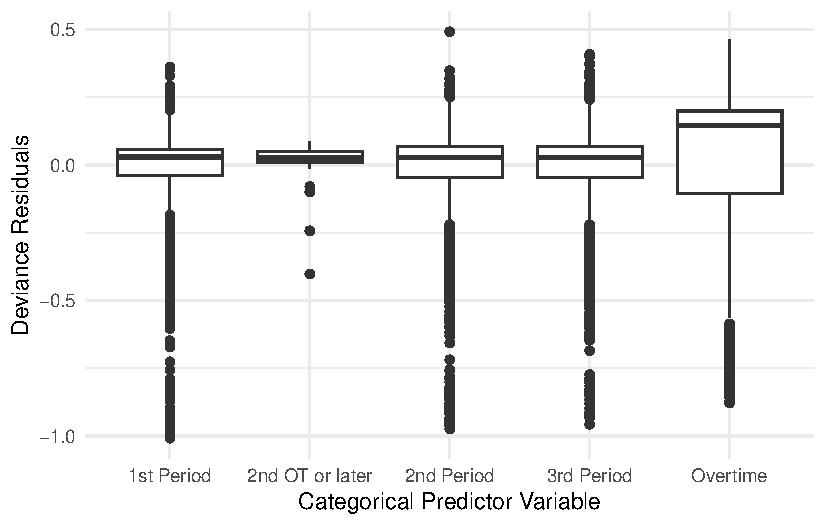
\includegraphics[width=0.5\textwidth,height=\textheight]{paper_files/figure-pdf/unnamed-chunk-28-1.pdf}

\begin{verbatim}
Warning: `aes_string()` was deprecated in ggplot2 3.0.0.
i Please use tidy evaluation idioms with `aes()`.
i See also `vignette("ggplot2-in-packages")` for more information.
\end{verbatim}

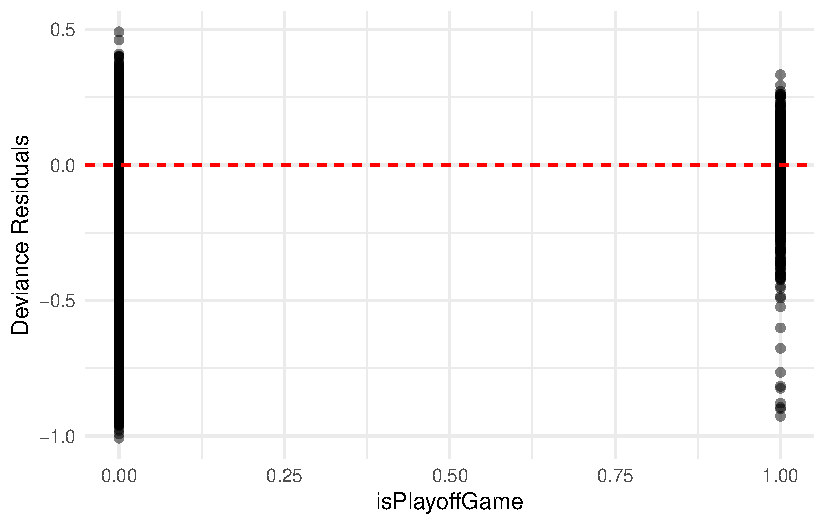
\includegraphics[width=0.5\textwidth,height=\textheight]{paper_files/figure-pdf/unnamed-chunk-29-1.pdf}

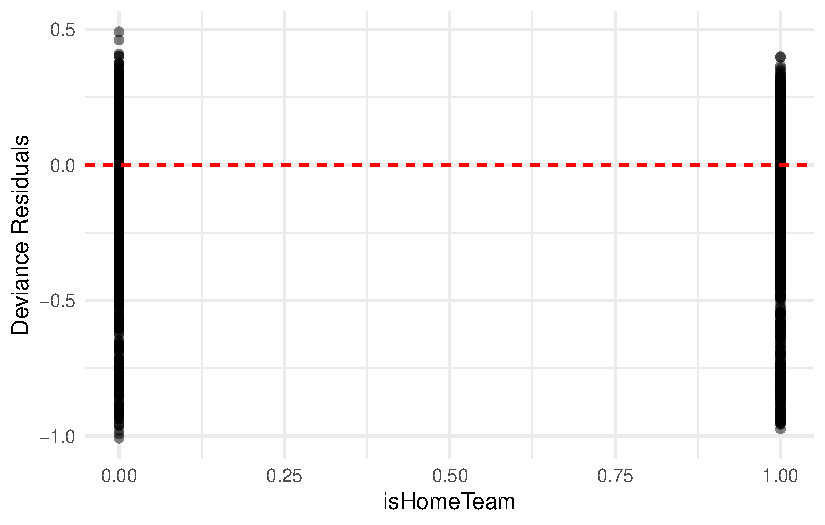
\includegraphics[width=0.5\textwidth,height=\textheight]{paper_files/figure-pdf/unnamed-chunk-30-1.pdf}

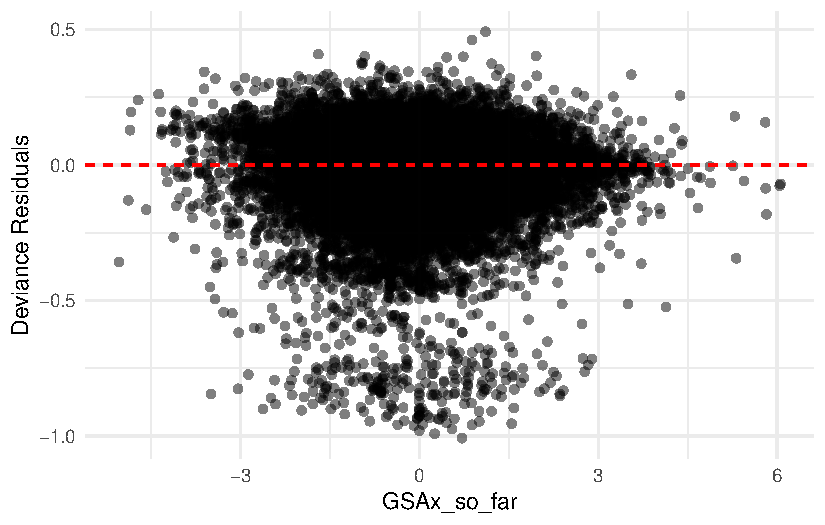
\includegraphics[width=0.5\textwidth,height=\textheight]{paper_files/figure-pdf/unnamed-chunk-31-1.pdf}

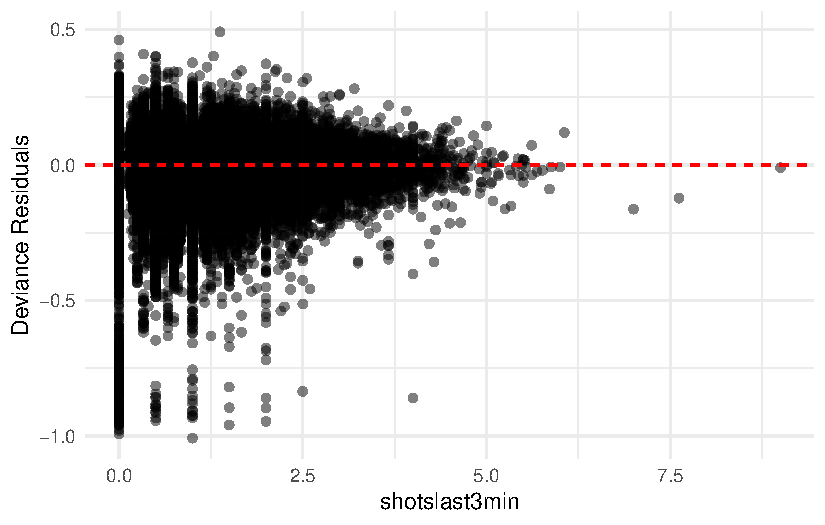
\includegraphics[width=0.5\textwidth,height=\textheight]{paper_files/figure-pdf/unnamed-chunk-32-1.pdf}

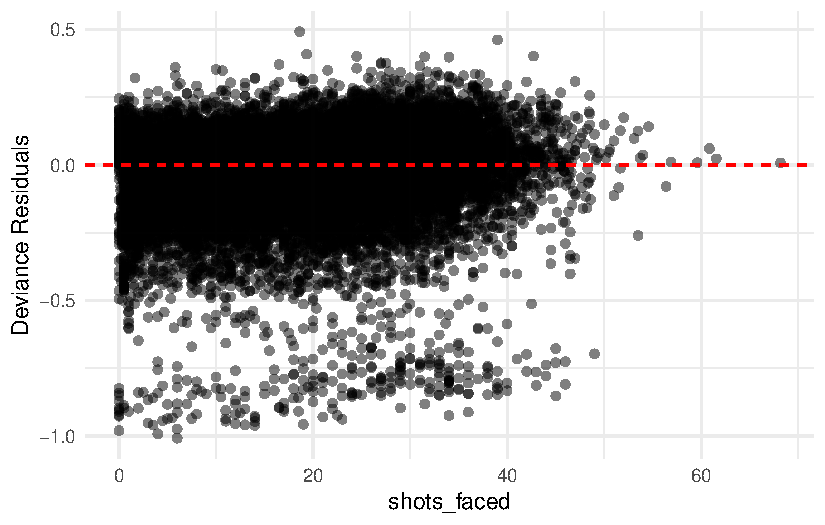
\includegraphics[width=0.5\textwidth,height=\textheight]{paper_files/figure-pdf/unnamed-chunk-33-1.pdf}

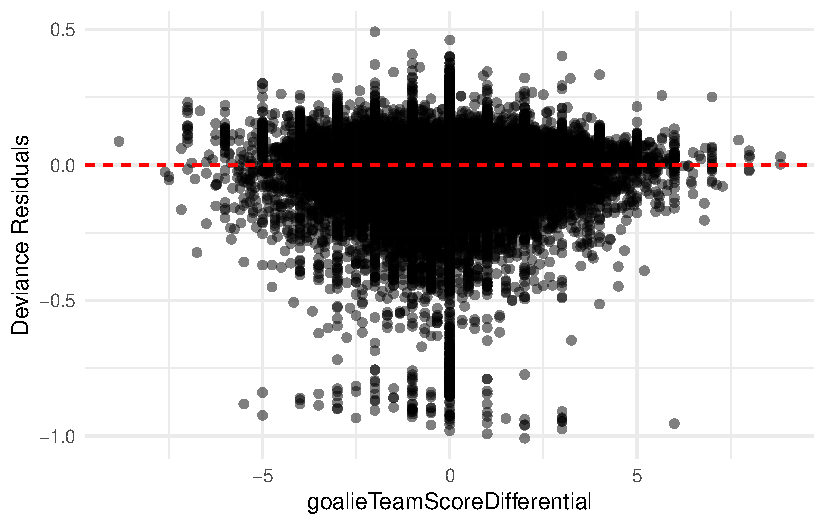
\includegraphics[width=0.5\textwidth,height=\textheight]{paper_files/figure-pdf/unnamed-chunk-34-1.pdf}

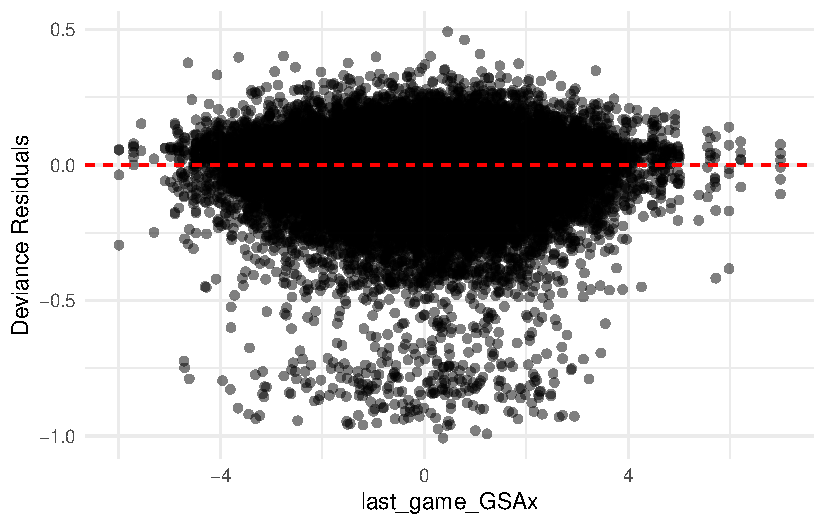
\includegraphics[width=0.5\textwidth,height=\textheight]{paper_files/figure-pdf/unnamed-chunk-35-1.pdf}

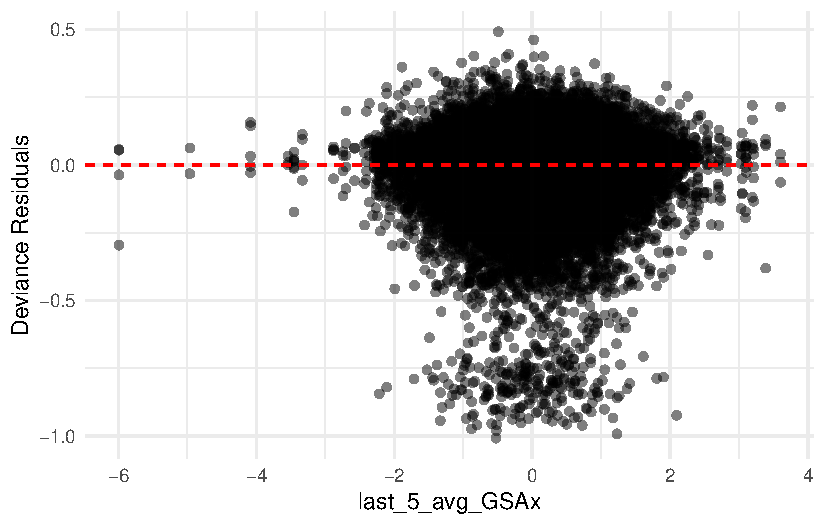
\includegraphics[width=0.5\textwidth,height=\textheight]{paper_files/figure-pdf/unnamed-chunk-36-1.pdf}

\subsubsection{Normal Q-Q plot to check
normality}\label{normal-q-q-plot-to-check-normality}

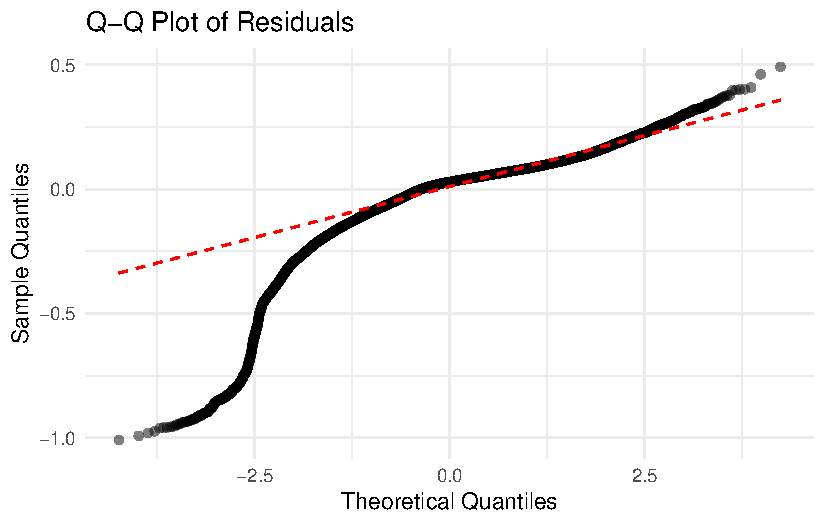
\includegraphics[width=0.5\textwidth,height=\textheight]{paper_files/figure-pdf/unnamed-chunk-37-1.pdf}

\newpage

\section*{References}\label{references}
\addcontentsline{toc}{section}{References}

\phantomsection\label{refs}
\begin{CSLReferences}{1}{0}
\bibitem[\citeproctext]{ref-sportradar}
2024. \emph{Sportradar}.
\url{https://developer.sportradar.com/ice-hockey/reference/nhl-overview}.

\bibitem[\citeproctext]{ref-modelsummary}
Arel-Bundock, Vincent. 2022. {``{modelsummary}: Data and Model Summaries
in {R}.''} \emph{Journal of Statistical Software} 103 (1): 1--23.
\url{https://doi.org/10.18637/jss.v103.i01}.

\bibitem[\citeproctext]{ref-homeadv}
Bischof, Zachary. 2021. {``How Significant Is Home Advantage in the
NHL?''} \url{https://www.zbischof.com/hockey/2021-03-01-home-adv/}.

\bibitem[\citeproctext]{ref-playoffs}
Donchess, Jeff. 2022. {``NHL Scoring Trends: Regular Season Vs.
Playoffs.''} \emph{DRatings}.
\url{https://www.dratings.com/nhl-scoring-trends-regular-season-vs-playoffs/}.

\bibitem[\citeproctext]{ref-datasheet}
Gebru, Timnit, Jamie Morgenstern, Briana Vecchione, Jennifer Wortman
Vaughan, Hanna Wallach, Hal Daumé III, and Kate Crawford. 2018.
{``Datasheets for Datasets.''}
\url{https://www.microsoft.com/en-us/research/uploads/prod/2019/01/1803.09010.pdf}.

\bibitem[\citeproctext]{ref-caret}
Kuhn, and Max. 2008. {``Building Predictive Models in r Using the Caret
Package.''} \emph{Journal of Statistical Software} 28 (5): 1--26.
\url{https://doi.org/10.18637/jss.v028.i05}.

\bibitem[\citeproctext]{ref-citeR}
R Core Team. 2023. \emph{{R: A Language and Environment for Statistical
Computing}}. Vienna, Austria: R Foundation for Statistical Computing.
\url{https://www.R-project.org/}.

\bibitem[\citeproctext]{ref-arrow}
Richardson, Neal, Ian Cook, Nic Crane, Dewey Dunnington, Romain
François, Jonathan Keane, Dragoș Moldovan-Grünfeld, Jeroen Ooms, Jacob
Wujciak-Jens, and Apache Arrow. 2024. \emph{Arrow: Integration to
'Apache' 'Arrow'}. \url{https://github.com/apache/arrow/}.

\bibitem[\citeproctext]{ref-moneypuck}
Tanner, Peter. 2024. {``Moneypuck Shot Data.''} \emph{MoneyPuck}.
\url{https://moneypuck.com/data.htm}.

\bibitem[\citeproctext]{ref-testthat}
Wickham, Hadley. 2011. {``Testthat: Get Started with Testing.''}
\emph{The R Journal} 3: 5--10.
\url{https://journal.r-project.org/archive/2011-1/RJournal_2011-1_Wickham.pdf}.

\bibitem[\citeproctext]{ref-tidyverse}
Wickham, Hadley, Mara Averick, Jennifer Bryan, Winston Chang, Lucy
D'Agostino McGowan, Romain François, Garrett Grolemund, et al. 2019.
{``Welcome to the {tidyverse}.''} \emph{Journal of Open Source Software}
4 (43): 1686. \url{https://doi.org/10.21105/joss.01686}.

\bibitem[\citeproctext]{ref-knitr}
Xie, Yihui. 2014. {``{knitr}: A Comprehensive Tool for Reproducible
Research in {R}.''} In \emph{Implementing Reproducible Computational
Research}, edited by Victoria Stodden, Friedrich Leisch, and Roger D.
Peng. Chapman; Hall/CRC.

\bibitem[\citeproctext]{ref-zoo}
Zeileis, Achim, and Gabor Grothendieck. 2005. {``Zoo: S3 Infrastructure
for Regular and Irregular Time Series.''} \emph{Journal of Statistical
Software} 14 (6): 1--27. \url{https://doi.org/10.18637/jss.v014.i06}.

\bibitem[\citeproctext]{ref-kableExtra}
Zhu, Hao. 2021. \emph{kableExtra: Construct Complex Table with 'Kable'
and Pipe Syntax}. \url{https://CRAN.R-project.org/package=kableExtra}.

\end{CSLReferences}




\end{document}
